
BWA-MEM is a popular DNA read mapper used in many real-life applications. Its name stands for \emph{Burrows-Wheeler Aligner - Maximal Exact Match}. In this section, we will provide details of the BWA-MEM algorithms.

\subsection{Considerations about mapping and alignment}
First, we will start with some definitions. \emph{Mapping} is the process of finding correspondence between a data set of DNA fragments called "reads" and a reference genome. To do so, for each read, we first find small areas where the read exactly matches somewhere in the reference genome. This is the \emph{seeding} phase. Then, for all seeds, a \emph{seed-extension} is performed. 

After seeding, overlapping seeds or seeds that are close enough in the reference are grouped into \emph{chains}. This allows to fetch a single area in the reference to perform the mapping with the read. The area fetched is larger than the read, since there may be deletions in the read.

When we have a read and a segment of the reference with a corresponding seed, we perform the \emph{seed-extension}, which consists in two alignments on both left and right sides of the seed. If the seed is located at the beginning or the end of the read, only one seed-extension is performed (there is nothing to extend if the seed is on the border). In the extension process, we call \emph{query} the string coming from the read, and \emph{target} the one from the reference. When both sides of the seed must be aligned, we have then a left query to align with a left target, and a right query to align with the right target.

BWA-MEM operates in three major steps~\cite{li:bwamem}: seeding, chaining, and seed-extension. We will detail these three phases.

\subsection{Seeding}
\emph{Seeding} consists in finding small areas in the read that exactly match in the reference. This search is done with an FM-index.

The FM-index is a compressed representation for the reference genome. It is widely used due to its lightweight memory footprint, which is sub-linear with respect to the size of the data. Searching for a pattern in the compressed text is also sub-linear in time, which makes it ideal for seeding. When a seed is located, a chunk is taken from the genome around the seed to perform the alignment with the query sequence. This chunk should be larger than the query with which it shares a seed, since there could be gaps in the alignment. More details are available online~\cite{wiki:FMIndex}, but the following work does not rely on how FM-index works. 

When finding seeds, multiple areas can overlap in the read and the reference, or some seeds can be contained in others. To produce the most useful results, BWA-MEM produces seeds that have two characteristics:
\begin{itemize}
    \item they cannot be extended any further,
    \item each seed is not contained in any other seed of the read.
\end{itemize}
These seeds are called Super-maximal Exact Matches, or \emph{SMEM}s\cite{li:smem}.

\subsection{Chaining}
During seeding, multiple seeds can be found in various parts of the reference genome, and depending on how they overlap, they can be grouped in chains. Colinear seeds, or seeds very close to each other are grouped. Very small seeds, or seeds largely contained in longer seeds are filtered out. This heuristics reduces the number of seeds to extend by only keeping the most valuable ones. Seeding and chaining are shown in Figure~\ref{fig:poster-seeding}. In this example, the dark-blue seed has been found as substring of the red string in the query. But since it is long enough to be considered and close enough to the already existing light-blue seed, these two seeds are grouped in a chain, as shown at the bottom of the Figure. The light blue seed is extended and its extension reaches the dark-blue seed. This is taken into account, and the dark-blue seed is not extended since it is contained in the alignment of the light-blue seed.

\begin{figure}
    \centering
    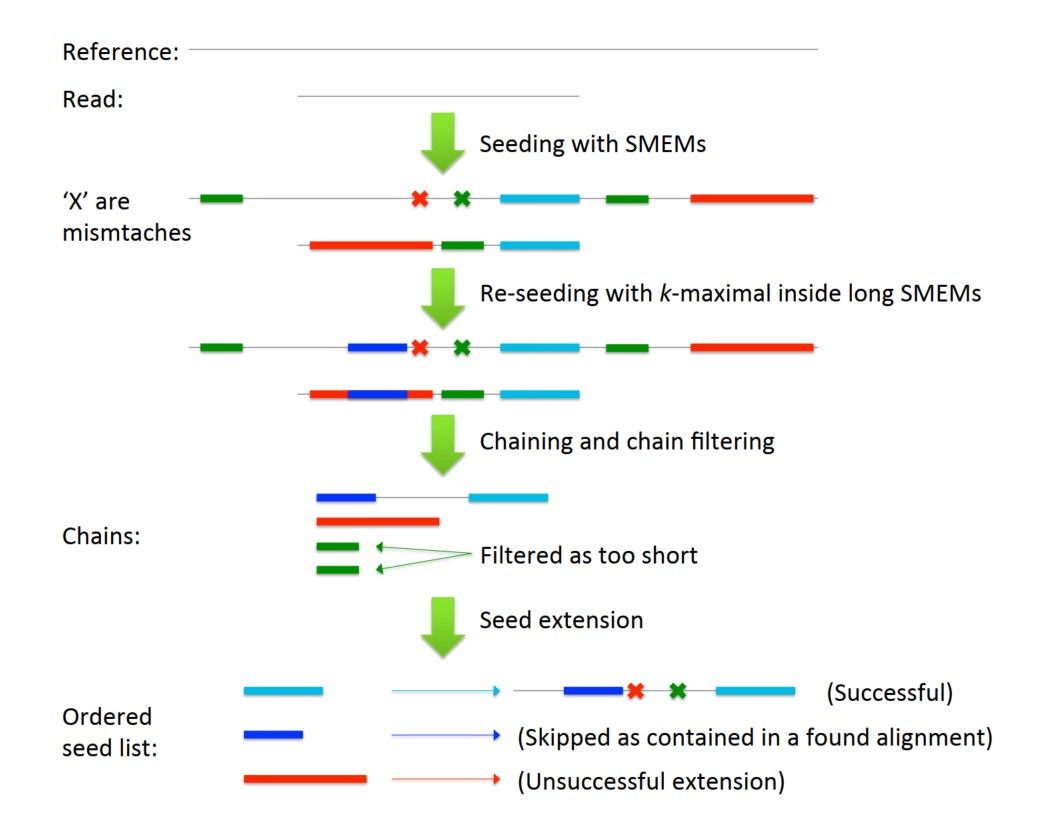
\includegraphics[width=0.9\linewidth]{poster_seeding}
    \caption{Seeding process along with chaining. (from~\cite{poster:bwa})}
    \label{fig:poster-seeding}
\end{figure}{}

When starting extension, seeds are ordered by decreasing score of their chain. Seeds within longest chains are aligned first, since they have a high probability of reaching other seeds of their chains when aligned.

\subsection{Seed-extension}
\label{sec:local}
After seeding, we have to continue to align on both sides of the seed. 

%\warn{Here provide the detal how a reagion is extracted from the referene genome to be aligned with the read and which alignment algorithm is used i.e. Blast-like seed extension. Use the Blast-like seed extension algorithm in [24] and modify it if it is different from actually used in BWA-MEM. Use the figures in BWA-MEM poster}

We define a match score corresponding to the score when two bases are equal. In the case of mismatches, they can appear in the form of insertion or deletion of one or multiple bases, in either the read or the reference. We then define an insertion mismatch score and a deletion mismatch score. The matching score has a positive value, and the mismatch scores are negative, and often both insertion and deletion mismatch scores are set at the same value. For the query sequences, it may happen that a base cannot be correctly retrieved by the sequencing machine, and if this happens, the unknown base is denoted as "N" and is always counted as a mismatch. Furthermore, in real-life mutations, it is much more likely to have a small number of long gaps rather than multiple short gaps. To reflect this, the model "affine gap penalty" for DNA mutation is used. We define a big mismatch score for opening a gap, and a smaller mismatch score for extending the gap. This way, during the alignment, we apply a bigger penalty when trying to open a gap rather than when a mismatch only causes a gap to get wider. 

For extension, dynamic programming algorithms are used. They are compute-intensive (and compute-bound), but they provide an optimal solution to the alignment problem. We could actually use them to compute the whole alignment but it is much more efficient to run smaller alignments as left and right extensions of the seed. They rely on computing a matrix of size $N \times M$, $N$ and $M$ being the length of the query and target sequences respectively. As shown in Figure~\ref{fig:dpmatrix}, we place the target sequence as a row, and the query as a column. Each cell is filled with a score depending on the north cell, the west cell, and the north-west cell, and the current bases to align. For the pair of bases, it corresponds to row and the column. We assume that we count matches with a score $\alpha > 0$, mismatches with a score $\beta < 0$, and a score for insertion and deletion $\gamma < 0$. For affine gap penalty, we need to differentiate when the alignment opens a gap and when it expands a gap. To this end, we define $g < 0$ as score applied to open a gap, and $h < 0$ as score applied when expanding an existing gap. We have $|g| > |h|$ as opening a gap should be more costly than widening it. Equation~\ref{equ:gapa} defines the score to apply when opening or widening a gap in the query, and Equation~\ref{equ:gapb} shows the same for target. We define the relation for the score $S[i,j]$ on cell $i,j$ related to bases $a_i$ and $b_j$ with affine gap penalty in Equation~\ref{equ:dp}.

In the example in Figure~\ref{fig:dpmatrix}, we have $\alpha = 2$ and $\beta = \gamma = -1$. More detailed information can be found in ~\cite{Aluru:2005:HCM:1121650}.

\begin{equation}
 	S[i,j] = max \left\{
 	\begin{array}{llll}
 		S[i-1, j-1] + \alpha & \mbox{if} & a_i = b_j \\
 		S[i-1, j-1] + \beta & \mbox{if} & a_i \neq b_j \\
 		G_{A}[i,j] \\
 		G_{B}[i,j]\\
 	\end{array}
 	\right.
 	\label{equ:dp}
 \end{equation}
 \begin{equation}
 	G_{A}[i,j] = max \left\{
 	\begin{array}{ll}
 		S[i-1, j] + g + h \\
 		G_{A}[i-1,j] + h \\
 		 
 	\end{array}
 	\right.
 	\label{equ:gapa}
 \end{equation}
  \begin{equation}
 	G_{B}[i,j] = max \left\{
 	\begin{array}{ll}
 		S[i, j-1] + g + h \\
 		G_{B}[i,j-1] + h \\
 		 
 	\end{array}
 	\right.
 	\label{equ:gapb}
 \end{equation}
 
 \begin{figure}[ht!]
 	\centering
 	\begin{subfigure}[t]{0.5\textwidth}
 		\centering
 		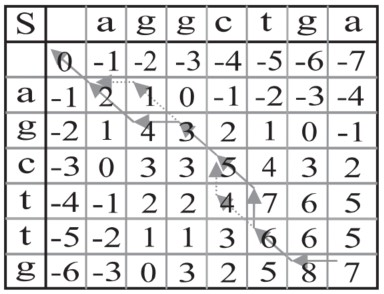
\includegraphics[height=0.5\textwidth]{global_align}
 		\caption{Global alignment}
 		\label{fig:global_align}
 	\end{subfigure}%
 	~ 
 	\begin{subfigure}[t]{0.5\textwidth}
 		\centering
 		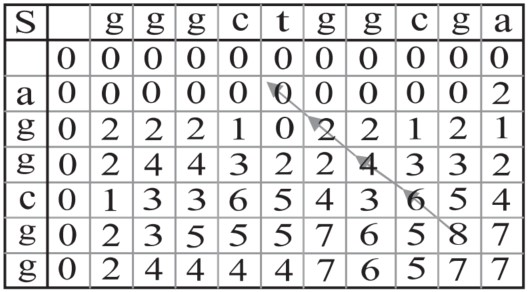
\includegraphics[height=0.5\textwidth]{local_align}
 		\caption{Local alignment}
 		\label{fig:local_align}
 	\end{subfigure}
 	\caption{Dynamic programming alignments (from ~\cite{Aluru:2005:HCM:1121650}) }
 	\label{fig:dpmatrix}
 \end{figure}

Among dynamic programming (DP) algorithms, we can cite main techniques:

 \begin{itemize}
 	\item Needleman-Wunsch~\cite{NeedlemanWunsch:method}, or \emph{global} alignment: it tries to match the whole sequences. The results contains both sequences completely, as Figure~\ref{fig:global_align} shows, with the alignment path traversing the matrix. Mismatches on ends cause a penalty, as shows the negative scores on the edges;
	\item Smith-Waterman~\cite{SmithWaterman:identification}, or \emph{local} alignment: it aligns two sequences but only looks for the maximal score, which reports the best alignment there is. On Figure~\ref{fig:local_align}, one can see we select the best score, the score is initialised at 0 and stays positive;
	\item A mix of the two, \emph{semi-global}~\cite{Durand:course-genomics} alignment, that performs a global alignment but allows to skip both ends of the query sequence. In practical, semi-global is often used instead of global;
	\item BLAST~\cite{Altschul:BLAST}-like extension: it performs two alignments on both ends of the chain instead of aligning the sequences entirely. If first makes a local alignment on the left side, starting with a non-zero score, but taking the chain score instead. Then it makes a local alignment on the right side, starting as initial score the previous computed score (taking the chain and left alignment). This splits the alignment problem in two, which makes it much faster. This is the technique used in seed-extension.
\end{itemize}

The pseudocode for local alignment is presented in Algorithm~\ref{algo:local}. It computes the whole dynamic programming matrix $S$ with the equation~\ref{equ:dp} showed above. There are small difference between global, local and semi-global alignments in the initialisation step, the computing formula, and how the final score is obtained from the matrix. For the local alignment, which is the one we will use in the rest of the thesis, initialisation is done with a score of zero along both north and west edges of the matrix. This means that no penalty is made on the ends of both sequences. Second, in the computing formula showed in equation~\ref{equ:dp}, the score can actually go negative if a lot of mismatches occur. We do not want this behaviour with local alignment, meaning that there is no penalty if an area is not aligned (the alignment can occur later on in the sequence). In Algorithm~\ref{algo:local}, this is shown by taking the maximum of the computed score with 0. Finally, in local alignment, we want the best possible score without constraints on the end of the alignment, so we simply take the maximum value in the dynamic programming matrix as the end position of the alignment.

 \begin{algorithm}[h!]
 	\caption{Dynamic programming matrix computation algorithm}
 	\label{algo:local}
 	\begin{algorithmic}[1] % The number tells where the line numbering should start
 		\Procedure{Compute the dynamic programming matrix, local alignment}{$query\_string$, $target\_string$, $query\_length$, $target\_length$} \Comment{}
		

 		\State \emph{Initialise score}
 		\For{i from -1 to $query\_length$}
 			\State $S_{i, -1} \leftarrow 0$
 		\EndFor	
				
 		\For{j from -1 to $target\_length$}
 			\State $S_{-1, j} \leftarrow 0$	
 		\EndFor

 		\State \emph{compute S matrix}
 		\For{ (i from $0$ to $query\_length - 1$}
 			\For {j from $0$ to $target\_length - 1$}

 				\State Read base $query\_base_i$ in $query\_string$
 				\State Read base $target\_base_j$ in $target\_string$ 	
 				\State $ 	S_{i,j} \leftarrow max \left\{
 				\begin{array}{llll}
 				S_{i-1, j-1} + \alpha & \mbox{if} & query\_base_i = target\_base_j \\
 				S_{i-1, j-1} + \beta & \mbox{if} & query\_base_i \neq target\_base_j \\
 		 		G_{A}[i,j] \\
 		        G_{B}[i,j]\\
 				0 \\
 				\end{array}
 				\right. $
				
 			\EndFor
			
 		\EndFor
		
 		\State Find $i_{max}$ and $j_{max}$ for which $S_{i_{max}, j_{max}} = max(S_{i,j})$
 		\State $score \leftarrow S_{i_{max}, j_{max}}$
 		\State $end\_position\_query \leftarrow i_{max}$
 		\State $end\_position\_target \leftarrow j_{max}$
	
 		\EndProcedure
		
	\end{algorithmic}
\end{algorithm}

Another optimisation called \emph{z-dropoff} is interrupting the calculation of a row when the score drops sharply. This is meant to stop computing as soon as the sequences are visibly not aligned anymore. As shown in Figure~\ref{fig:zdrop}, the goal is to avoid finding a matching area after a non-matching one, since it does not bear any biological meaning and the next aligned region could simply be another seed.

\begin{figure}[h!]
    \centering
    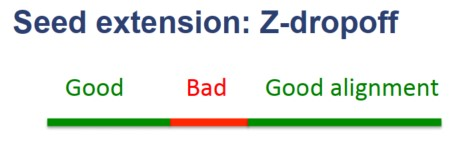
\includegraphics[width=0.6\linewidth]{zdrop}
    \caption{Z-dropoff use case: when a badly matching region is found between two matching alignments. (from~\ref{fig:poster-seeding})}
    \label{fig:zdrop}
\end{figure}{}

Finally, it can be noticed that the north-east and south-west corners of the dynamic programming matrix are often useless to compute, since reaching these cells would mean that the alignment is containing a huge gap (and hence has a mediocre score). One can simply avoid to compute them, resulting in only calculating a band around the diagonal, hence calling this technique \emph{banded} dynamic programming.

\subsection{BWA-MEM output}

BWA-MEM outputs the alignments in the Sequence Alignment Mapping~\cite{samtools:sam} (SAM) format. It is a text-based format with fields separated by tabulations. The first eleven fields are mandatory and Table~\ref{tab:samformat} describes them. In particular, the 5$^{th}$ field "Mapping quality" describes how good the obtained mapping is. In downstream analysis, low-quality mapping are often filtered out using the value of this field. The threshold usually taken for filtering is 20: mapping with a quality strictly lower than 20 are removed.

\begin{figure}[h!]
    \centering
    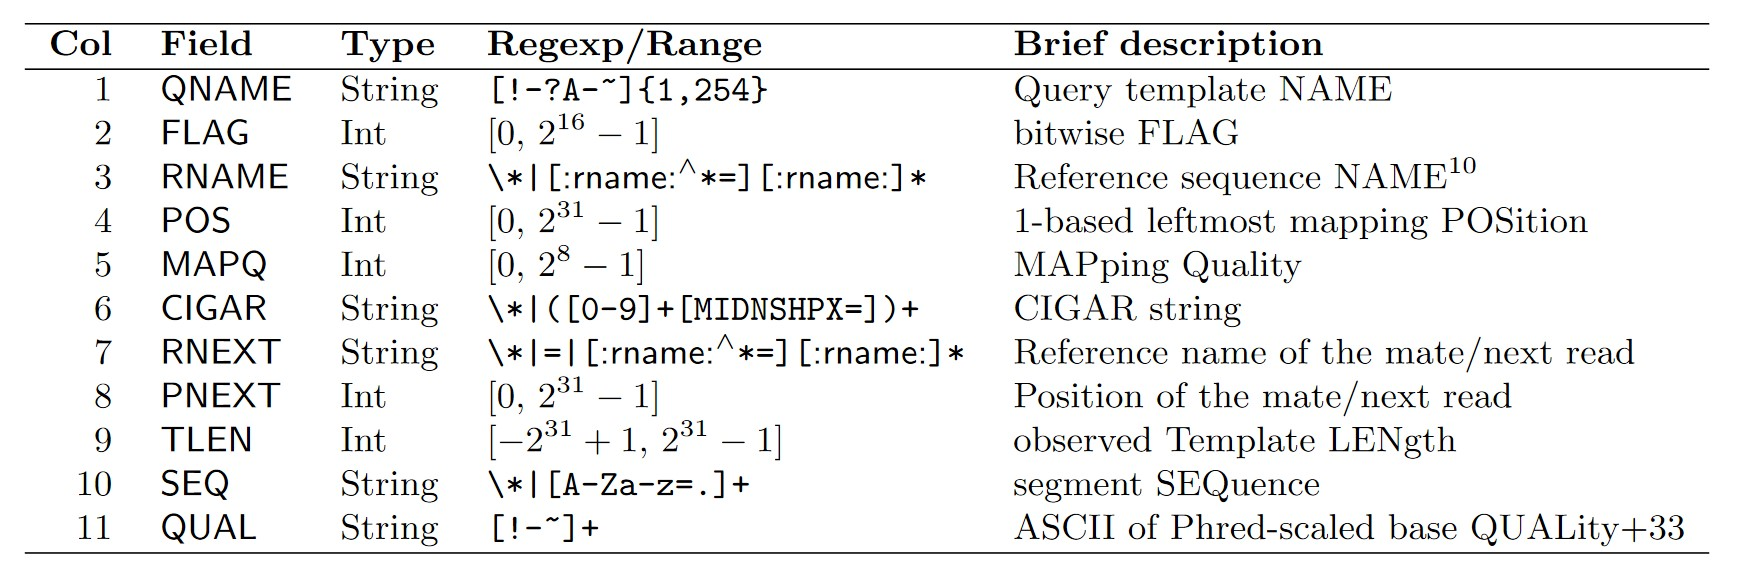
\includegraphics[width=1\linewidth]{samformat}
    \captionof{table}{The mandatory fields for SAM format. (from~\cite{samtools:sam})}
    \label{tab:samformat}
\end{figure}{}

BWA-MEM outputs in the 6$^{th}$ field the \emph{CIGAR string}, which is a compact way to write the alignment, and describes the way the read maps with the reference. Each letter bears a meaning concerning the alignment. They are presented in Table~\ref{tab:cigar}. Each number before a letter means how many times the next letter is applied. For example, a CIGAR string of \verb|100M3D12I| means that the first 100 bases of the read are matching, then the 3 next bases are deletions (gaps in the target), then the next 12 bases are insertions (gap in the query). In the table, "consumes query" and "consumes target" is a way to define if, when reading the CIGAR string, one should go forward in the target or query DNA string.

\begin{figure}[h!]
    \centering
    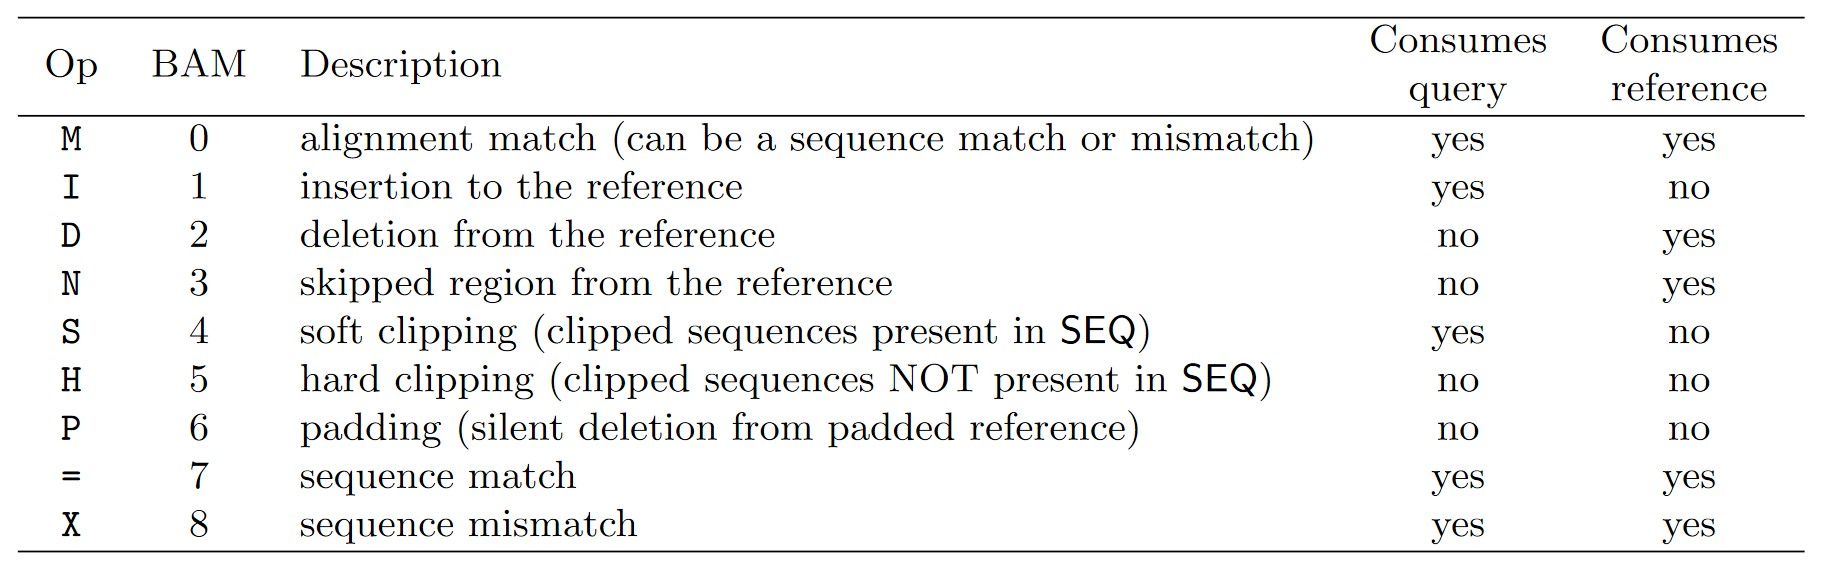
\includegraphics[width=1\linewidth]{cigarguide}
    \captionof{table}{The CIGAR string components. (from~\cite{samtools:sam})}
    \label{tab:cigar}
\end{figure}{}

